\documentclass[a4paper,11pt, notitlepage ]{article}
\usepackage[T1]{fontenc}
\usepackage[polish]{babel}
\usepackage[utf8]{inputenc}
\usepackage{lmodern}
\usepackage{enumitem}
\usepackage{indentfirst}
\usepackage{graphicx}
\usepackage{wrapfig}
\usepackage{fancyhdr}
\usepackage{lastpage}
\pagestyle{fancy}
\fancyhf{}
\setcounter{page}{1}
\rfoot{Strona \thepage \hspace{1pt} z \pageref{LastPage}}
\selectlanguage{polish}
\makeatletter
\newcommand{\linia}{\rule{\linewidth}{0.4mm}}
\renewcommand{\maketitle}{\begin{titlepage}
    \vspace*{1cm}
    \begin{center}\small
    Politechnika Warszawska\\
    Wydział Elektryczny
    \end{center}
    \vspace{3cm}
    \noindent\linia
    \begin{center}
      \LARGE \textsc{\@title}
         \end{center}
     \linia
    \vspace{0.5cm}
    \begin{flushright}
    \begin{minipage}{8cm}
    \textit{\small Autorzy:}\\
    \normalsize \textsc{\@author} \par
    \end{minipage}
    \end{flushright}
    \vspace*{\stretch{6}}
    \begin{center}
    \@date
    \end{center}
  \end{titlepage}%
}
\makeatother
\author{J.~Korczakowski, nr albumu 291079\\ B.~Suchocki, nr albumu 291111\\ Grupa projektowa nr 11}
\title{Specyfikacja funkcjonalna symulatora automatu komórkowego \textsl{Life}}
\frenchspacing
\begin{document}
\maketitle
\setcounter{page}{2}
\section{Opis ogólny}
\subsection{Nazwa programu}
Nasz program będzie nazywał się \verb+AutomatKomorkowyLIFE+.
\subsection{Poruszany problem}
Zadaniem naszego programu będzie symulacja automatu komórkowego Life, czyli symulacja popularnej „Gry w życie” wymyślonej przez Johna Conwaya w 1970 roku. Gra toczy się na planszy podzielonej na kwadratowe komórki. Każda z komórek może znajdować się w stanie martwym lub żywym. Przy przejściu do następnej generacji komórek, każda z nich może przeżyć, umrzeć lub ożyć w zależności od bieżącego stanu jej sąsiadów. Przyjmujemy, że komórka ma 8 (sąsiedztwo Moore’a) lub 4 (sąsiedztwo von Neumanna) sąsiadów, w zależności od przyjętych zasad sąsiedztwa. To, ile żywych sąsiadów musi mieć komórka, aby przeżyć, umrzeć lub ożyć określają możliwe do zmiany zasady gry.
\newline \indent Dodatkowo, w naszym programie zakładamy, że plansza jest ograniczona i komórki poza nią są martwe. Naszym zdaniem uprości to symulację i zwiększy jej czytelność.
\subsection{Cel projektu}
Celem tego projektu jest nauka i praktyka programowania w języku C~przy jednoczesnym zapoznaniu się z tematem symulacji automatu komórkowego.
\section{Opis funkcjonalności}
\subsection{Korzystanie z programu}
Program uruchamiany jest z wiersza poleceń. Obok nazwy programu użytkownik może podać dodatkowe parametry.
\subsection{Uruchomienie}
Ogólny schemat polecenia do uruchomienia programu:
\begin{verbatim}
./AutomatKomorkowyLIFE [-i plik_konfig] [-g ile_ generacji] 
[-o plik_wyjsciowy]
\end{verbatim}

Gdzie: 
\begin{itemize}
\item \verb+plik_konfig+ – plik wejściowy konfiguracyjny (opisujący stan początkowej generacji),
\item \verb+ile_generacji+ – liczba (naturalna) generacji do przeprowadzenia,
\item \verb+plik_wyjsciowy+ – plik wyjściowy opisujący konfigurację ostatniej generacji (po symulacji),
\item \verb+ile_obrazow+ – liczba obrazów przedstawiających stan wybranych generacji.
\end{itemize}
\subsection{Możliwości programu:}
\begin{itemize}
\item zmiana obowiązujących podczas symulacji zasad sąsiedztwa,
\item przeprowadzenie symulacji automatu komórkowego na podstawie wczytanego pliku konfiguracyjnego i zasad sąsiedztwa,
\item wyświetlanie bieżących generacji na standardowe wyjście,
\item wygenerowanie obrazów *.png przedstawiających stan wybieranych na bieżąco przez użytkownika generacji,
\item wygenerowanie pliku wyjściowego opisującego stan ostatniej generacji.
\end{itemize}
\section{Format danych i struktura plików}
\subsection{Pojęcia}
\begin{description}
\item[Komórka] – podstawowa jednostka automatu komórkowego.
\item[Generacja] – jeden cykl, w którym komórki rodzą się lub umierają.
\item[Stan komórki] – komórka może znajdować się w dwóch stanach, żywym (włączonym) lub martwym(wyłączonym).
\item[Sąsiedzi komórki] – komórki przylegające do niej bokami i rogami (sąsiedztwo Moore’a) lub tylko bokami(sąsiedztwo von Neumanna).
\begin{figure}[h]
\centering
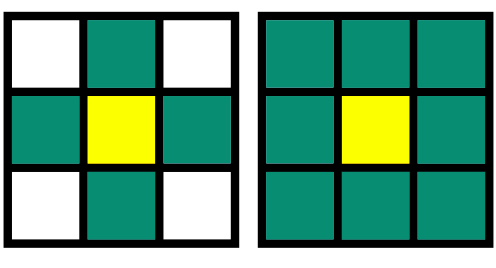
\includegraphics[width=7cm]{s}
\caption{Sąsiedztwo von Neumanna(po lewej) oraz Moore'a(po prawej).}
\end{figure}
\end{description}
\subsection{Struktura katalogów}
Projekt będzie znajdował się w katalogu \verb+Symulator+.  Pliki z kodem źródłowym i plikami nagłówkowymi znajdą się w~katalogu \verb+src+. W katalogu \verb+data+ umieścimy domyślny plik wejściowy. Dane testowe będą znajdowały się w~katalogu \verb+test+ w katalogu \verb+data+. Wyniki działania naszego programu(plik wyjściowy i pliki .png) umieścimy w katalogu \verb+bin+. W katalogu głównym naszego projektu znajdzie się również plik \verb+Makefile+.

Graficzne przedstawienie struktury katalogów w naszym projekcie:
\begin{verbatim}
Symulator
+--- src
+--- data
|    +--- test
+--- bin
+--- Makefile
\end{verbatim}
\subsection{Przechowywanie danych w programie}
 Plansza przeznaczona do symulacji będzie trzymana w strukturze. Wyróżnimy w niej pola takie jak, dwuwymiarowa tablica typu \verb+char+ oraz jej szerokość i wysokość.
\subsection{Dane wejściowe}
 Plik wejściowy konfiguracyjny zawiera w pierwszym wierszu szerokość s~i~wysokość w planszy a w kolejnych w wierszach po s zer i jedynek. Liczba 0 odpowiada martwej komórce, a 1 żywej.

Plik ustawień zawiera w pierwszym wierszu literę M lub N (domyślnie M), odpowiadającą użytej zasadzie sąsiedztwa (Moore’a lub von Neumanna), a w drugim wierszu opis ustawień reguł „gry w życie” w formacie $x_{1}x_{2}$ \ldots $x_{n}$ /$y_{1}y_{2}$\ldots $y_{m}$, gdzie $x_{1}x_{2}$\ldots $x_{n}$-liczby komórek w sąsiedztwie, dla których żywe komórki przeżywają, $y_{1}y_{2}$\ldots $y_{m}$ – liczby komórek w sąsiedztwie, dla których martwe komórki ożywają.
\subsection{Dane wyjściowe}
Pliki wyjściowe naszego programu dzielą się na dwa rodzaje. Jeden rodzaj to stan bieżącej generacji zapisany w formacie analogicznym do pliku wejściowego przyjmowanego przez nasz program. Drugi rodzaj to pliki .png zawierające obrazy generacji, których zażądał użytkownik.
\section{Scenariusz działania programu}
\subsection{Scenariusz ogólny}
\begin{enumerate}
\item Uruchomienie programu z wiersza poleceń.
\item Sprawdzenie parametrów wywołania.
\item Otwarcie plików: wejściowego konfiguracyjnego, ustawień oraz pliku wyjściowego.
\item Wygenerowanie planszy.
\item Symulacja podanej liczby generacji, wypisywanie bieżącej i ewentualne (decyduje o tym użytkownik) generowanie plików .png przedstawiających stan aktualnej generacji.
\item Wypisanie opisu ostatniej generacji do pliku wyjściowego.
\item Zakończenie działania programu.
\end{enumerate}
\subsection{Scenariusz szczegółowy}
\makeatletter
\renewcommand{\theenumii}{\@arabic\c@enumii}
\renewcommand{\labelenumii}{\theenumi.\theenumii}
\makeatother
\begin{enumerate}
\item Uruchomienie programu z wiersza poleceń
\item Sprawdzenie podanych przez użytkownika parametrów:
\begin{itemize}
\item Jeśli użytkownik nie poda nazwy wejściowego pliku konfiguracyjnego, przypisana zostanie nazwa pliku domyślnego\newline (\verb+generation_config+).
\item Jeśli użytkownik nie poda liczby generacji do zasymulowania, przypisana zostanie wartość domyślna (20). 
\item Jeśli parametr oznaczający liczbę generacji będzie błędny (np. będzie literą), program wypisze komunikat: \verb+Nieprawidłowa liczba+ \verb+generacji+ na standardowe wyjście i zakończy działanie.
\item Jeśli użytkownik nie poda nazwy pliku wyjściowego, przypisana zostanie wartość domyślna (\verb+last_generation_config+)
\item Jeśli użytkownik poda nieobsługiwany parametr (np. poprzedzony zamiast \verb+-g+ prefiksem \verb+-u+, program go zignoruje
\end{itemize}
\item Próba otwarcia plików: wejściowego konfiguracyjnego, ustawień oraz pliku wyjściowego
\begin{itemize}
\item Jeśli program nie będzie mógł otworzyć któregoś z pliku (np. przez brak uprawnień), wypisze komunikat: \verb+Nie można otworzyć+ \verb+pliku nazwa_pliku+ na standardowe wyjście i zakończy działanie.
\end{itemize}
\item Wygenerowanie planszy
\begin{enumerate}[label*=\arabic*.]
\item Alokacja pamięci potrzebnej do przechowywania planszy w strukturze.
\begin{itemize}
\item Jeśli wygenerowanie planszy będzie niemożliwe z powodu braku pamięci, program wypisze komunikat: \verb+Wygenerowanie planszy+ \verb+zakończone niepowodzeniem. Spróbuj podać mniejsze+ \\ \verb+rozmiary+ na standardowe wyjście i zakończy działanie.
\end{itemize}
\item Wypełnienie struktury przeprowadzone na podstawie zawartości wejściowego pliku konfiguracyjnego.
\begin{itemize}
\item Jeśli używany do generowania planszy plik wejściowy konfiguracyjny będzie w niewłaściwym formacie, program wypisze komunikat: \verb+Plik wejściowy nazwa_pliku jest+ \\\verb+w niewłaściwym formacie+ na standardowe wyjście i zakończy działanie.
\end{itemize}
\end{enumerate}
\item Symulacja podanej liczby generacji i równoległe generowanie obrazów przedstawiających stan wybranych przez użytkownika generacji.
\begin{itemize}
\item Jeśli plik ustawień ma błędny format, program zwróci komunikat: \verb+Błędny format pliku ustawień.+ na standardowe wyjście i zakończy działanie.
\end{itemize}
\begin{enumerate}[label*=\arabic*.]
\item Przejście do następnej generacji na podstawie zasad pobranych z~pliku ustawień i wypisanie jej stanu na standardowe wyjście.
\item Umożliwienie użytkownikowi podania komendy \verb+n+ lub \verb+s+.
\begin{itemize}
\item Jeżeli użytkownik poda jako komendę literę \verb+s+, program wygeneruje plik .png przedstawiający stan bieżącej generacji i~przejdzie do symulacji następnej generacji.
\begin{itemize}
\item Jeśli próba wygenerowania któregoś obrazu zakończy się niepowodzeniem, program wypisze komunikat o błędzie na standardowe wyjście, lecz nie zakończy działania.
\end{itemize}
\item Jeżeli użytkownik poda jako komendę literę \verb+n+, program od razu przeprowadzi symulację następnej generacji.
\item Jeżeli użytkownik wprowadzi komendę \verb+n liczba+, gdzie \verb+liczba+ jest liczbą całkowitą, program przeprowadzi symulację tylu generacji, ile wynosi \verb+liczba+, bez bieżącego wypisywania i~proszenia o wpisanie komendy.
\begin{itemize}
\item Jeśli \verb+liczba+ będzie większa od liczby pozostałych do zasymulowania generacji, program zasymuluje dokładnie taką ilość generacji, jaka pozostała do wykonania.
\end{itemize}
\item Jeżeli użytkownik poda inną komendę, program wypisze komunikat: \verb+Błędna komenda+ na standardowe wyjście i będzie czekać na podanie poprawnej.
\end{itemize}
\end{enumerate}
\item Wypisanie opisu ostatniej generacji do pliku wyjściowego
\item Zakończenie działania programu
\begin{enumerate}[label*=\arabic*.]
\item Wypisanie komunikatu: \verb+Program zakończył działanie+ na standardowe wyjście.
\end{enumerate}
\end{enumerate}
\section{Testowanie}
Działanie programu w wypadkach błędnie podawanych danych i parametrów przetestujemy podając na wejście (wcześniej przygotowane) błędnie sformatowane lub takie do których program nie ma uprawnień pliki i~nieprawidłowe parametry. Następnie przeanalizujemy jak zachowa się nasz program.

Moduł wczytywania macierzy, a także generowanie przez nasz program plików wyjściowych oraz .png sprawdzimy ręcznie, analizując to jak zachowa się nasz program. Działanie symulacji automatu komórkowego przetestujemy poprzez generację przez nasz program macierzy, która będzie znana przez nas z innych źródeł. Porównamy obie macierze i jeśli będą się różnić, to poprawimy nasz program.
\end{document}
